\documentclass{csri19}

%%% Starting page will be changed when we combine the proceedings
\setcounter{page}{3}

% PACKAGES ---------------------------------------------------------------
\usepackage{amsfonts,amsmath,graphicx,subfigure}
% ADD YOUR OWN PACKAGES HERE ---------------------------------------------
\usepackage{mathtools, amssymb}

% DEFINITIONS ------------------------------------------------------------
% ADD YOUR OWN DEFINITIONS HERE ------------------------------------------
% BE SURE TO PREFACE LABEL WITH YOUR OWN INITIALS (SSS in this example) --
\newcommand{\SSSnorm}[1]{\left\Vert#1\right\Vert}
\newcommand{\SSSabs}[1]{\left\vert#1\right\vert}
\newcommand{\CFKg}{\mathfrak{g}}

% This controls the table-of-contents entry in the proceedings. Edit it
% to include your article title followed by the authors' names, as shown.
\addcontentsline{toc}{chapter}{Exponential Integrators for the HOMME-NH
Nonhydrostatic Atmosphere Model\\
{\em C.F.\ Krause and A.J.\ Steyer}}

\pagestyle{myheadings}

\thispagestyle{plain}

% This gives the running head. Usually you list a shortened version of
% your article title (unless it's already very short) along with
% the author's names, as shown.
\markboth{Exponential Integrators for HOMME-NH}{C.F.\ Krause and A.J.\ Steyer}

% Put your article title in here
\title{Exponential Integrators for the HOMME-NH Nonhydrostatic Atmosphere
 Model}

% List each author, their affiliation, and their e-mail address, as shown.
\author{Cassidy F.\ Krause\thanks{University of Kansas, ckrause@ku.edu}
\and Andrew J.\ Steyer\thanks{Sandia National Laboratories, asteyer@sandia.gov}}

\begin{document}
\maketitle

% Include your abstract here.
\begin{abstract}
Time-stepping in the HOMME-NH nonhydrostatic atmosphere model requires 
integration of a stiff initial value problem. The current standard is to
 solve these equations using implicit-explicit Runge-Kutta (IMEX RK) 
methods with a horizontally explicit - vertically implicit (HEVI) 
partitioning. We introduce a horizontally explicit - vertically integrating
 factor exponential method (HEVI-Exponential) as an alternative to solving 
these stiff equations. The main drawback to exponential methods is the cost
 of forming the matrix exponential. Here, we show that we can mitigate this 
cost by taking advantage of the tridiagonal-like form of our Jacobian and 
parallelizing our computations, making this solver an attractive option for
HOMME-NH.
\end{abstract}

\section{Introduction} \label{CFK:sec:intro}
Stiff initial value problems, like the ones found in HOMME-NH, require a 
very small step size when solved explicitly. On the other hand, using a 
fully implicit method is computationally inefficient. To deal with these 
restrictions, two different approaches have been developed for solving 
stiff equations.

Consider an equation of the form \[ u_t = f(u) = s(u) + n(u),\] where $s(u)$ 
contains the stiff part of the equation, and $n(u)$ contains the nonstiff 
part. The current implementation in HOMME-NH uses an implicit Runge-Kutta
method on $s(u)$, and an explicit Runge-Kutta method to solve $n(u)$. This 
approach is efficient and accurate, but with recent advances in 
exponential-type integrators, it is worth examining their performance as 
well.

In this paper, we consider integrating factor Runge-Kutta methods (IFRKs). 
In this case, we split our method as \[ u_t = f(u_m) = L_mu_m + N(u_m),\] 
where $L_m$ is a linear operator containing the stiff part of the equation, 
and $N(u_m) = f(u_m)-L_mu_m$ contains the nonstiff terms. Often, 
$L_m = f'(u_m)$, but we do not assume this is the case. Using the change of
 variables $v(t) = e^{-L_m(t-t_m)}u(t)$, we have
\begin{equation}\label{CFK:eqn:vode}
v_t = e^{-L_m(t-t_m)}N(e^{L_m(t-t_m)}v).
\end{equation} 
We can now use a fully explicit $r-$stage Runge Kutta method to solve 
\ref{CFK:eqn:vode}.

The most expensive part of these IFRK methods is the formation of the 
matrix exponential. However, the structure of the Jacobian in HOMME-NH 
allows us to form these matrix exponentials efficiently and in parallel, 
making this a viable alternative to the IMEX Runge-Kutta methods.

The rest of the paper is structured as follows: In Section 
\ref{CFK:sec:matexp} we give a brief background of matrix exponentials; 
Sections \ref{CFK:sec:homme} and \ref{CFK:sec:ifrk} discuss the
implementation of Integrating Factor Runge-Kutta (IFRK) methods with the
HOMME-NH nonhydrostatic atmosphere model; and numerical results are given 
in Section \ref{CFK:sec:results}.

\section{Exponential Methods}\label{CFK:sec:matexp} 
While exponential integrators allow for a larger time step than explicit 
methods, a major drawback is the computational cost of forming the matrix
exponential. For this reason, matrix exponential methods were not widely 
used for many years, but advances in efficiently forming $e^A$ have 
recently made exponential methods competetive choices for numerical solvers.

The matrix exponential $e^A$ can be analytically computed if the matrix $A$
 is diagonalizable, but finding the eigenvalues of $A$ is expensive, and it
 is not generally guaranteed that $A$ is diagonalizable. A more general 
approach is to approximate $e^{A}$ using a Pad\'e or Taylor series 
approximation. Other methods of approximating the matrix exponential are 
discussed in \cite{CFK:Moler2003}.

We choose to implement a $(p,q)$-Pad\'e approximation 
$e^{A}\approx \left[Q_{pq}(A)\right]^{-1}P_{pq}(A)$, where $P_{pq}(A)$ and 
$Q_{pq}(A)$ are defined as follows:

\begin{align*}
P_{pq}(A) &= \sum_{j=0}^p\frac{(p+q-j)!p!}{(p+q)!j!(p-j)!}A^j\\
Q_{pq}(A) &= \sum_{j=0}^q\frac{(p+q-j)!q!}{(p+q)!j!(q-j)!}(-A)^j
\end{align*}

After we calculate the terms $P_{pq}$ and $Q_{pq}$, the product 
$e^A\approx\left[Q_{pq}(A)\right]^{-1}P_{pq}(A)$ is a potentially 
expensive computation because of the matrix inversion. Fortunately, for our
 application, the matrix $A$ we consider has a special structure that allows
us to approximate $e^A$ efficiently and accurately. This implementation is 
further discussed in Section \ref{CFK:sec:homme}.

The error for the $(p,q)$-Pad\'e approximation is given by
\[ e^A - \left[Q_{pq}(A)\right]^{-1}P_{pq}(A) = \mathcal{O}(A^{p+q+1}).\]

If the matrix $A$ has eigenvalues that are spread far apart, this 
approximation can be especially inaccuarate. To mitigate this problem, we 
implement a scaling and squaring approach. We briefly outline this 
procedure here; for further detail and error analysis of the scaling and 
squaring method, see \cite{CFK:higham2005} and \cite{CFK:Al-Mohy2009}. 

To scale $e^A$, we take advantage of the properties of matrix exponentials 
and write it as
\[e^{A} = \left(e^{A/k}\right)^k,\]
where we choose $k$ to be the smallest power of $2$ so that 
$\|A/k\| \leq 0.5$. With this factorization, the matrix $A$ is scaled down
 to $A/k$, and the matrix exponential $e^{A/k}$ is calculated using the 
Pad\'e formulas above. This matrix exponential is then squared repeatedly to 
recover the desired matrix exponential $e^{A}$.

\section{Implementation with HOMME-NH}\label{CFK:sec:homme}
HOMME-NH is a nonhydrostatic atmosphere model whose state variables are
listed in Table \ref{CFK:tab:variables}. The stiff terms in this model are 
$w$ and $\phi$, so we can write the governing equations as
\[q_t \coloneqq \begin{bmatrix} u_t \\
w_t\\
\phi_t\\
\theta_t\\
\frac{\partial \pi}{\partial \eta}
\end{bmatrix} = n(q) + s(q) \equiv n(q) + \begin{bmatrix}
0\\
-\CFKg (1-\mu)\\
\CFKg w\\
0\\
0\end{bmatrix}.\] 

\begin{table}[ht]
  \caption{Variables in HOMME-NH}
  \label{CFK:tab:variables}
  \begin{center}
    \begin{tabular}{|c|l|}
      \hline
      \textbf{Variable Name} & \textbf{Description} \\
      \hline
      $w$                                & Vertical velocity      \\
      $u$                                & Horizontal velocity    \\
      $\phi$                             & Geopotential           \\
      $\theta$                           & Potential temperature  \\
      $\frac{\partial\pi}{\partial\eta}$ &                        \\
      \hline
    \end{tabular}
  \end{center}
\end{table}

Linearizing $s(q)$ gives the following Jacobian:
\[ J = \begin{bmatrix}
0&                  &                                                   &  & \\
 & 0                & \CFKg \Delta t \frac{\partial \mu}{\partial \phi} &  & \\
 & \CFKg \Delta t I & 0                                                 &  & \\
 &                  &                                                   &0 & \\
 &                  &                                                   &  &0\end{bmatrix}.\]

So, forming $e^{\alpha J}$ reduces to forming an exponential of 
\[A \coloneqq \begin{bmatrix}
   0              & \CFKg \Delta t \frac{\partial \mu}{\partial \phi} \\
 \CFKg \Delta t I & 0  \end{bmatrix},\]
where $\dfrac{\partial \mu}{\partial \phi}$ is tridiagonal. This form 
allows us to solve $\left[Q_{pq}(A)\right]^{-1}P_{pq}(A)$ using 
tridiagonal solves and back substitution.

To do so, we first factor $Q_{pq}(A)$ as
\begin{align*}
Q_{pq}(A) &= \sum_{j=0}^q\frac{(p+q-j)!q!}{(p+q)!j!(q-j)!}(-A)^j\\
          &= \prod_{j=1}^q\left[\sigma_jI-A\right],
\end{align*}
where $\sigma_j\in \mathbb{C}$ for $j=1,\dots,q$.

Then, since we want to solve for 
$R \coloneqq \left[Q_{pq}(A)\right]^{-1}P_{pq}(A)$, we have
\begin{align*}
Q_{pq}(A) R &= P_{pq}(A)\\
\prod_{j=1}^q\left[\sigma_jI-A\right]R &= P_{pq}(A).
\end{align*}

Define $R_1 \coloneqq \left[\sigma_2I-A\right]\left[\sigma_3I-A\right]\cdots\left[\sigma_qI-A\right]R$.
Then our equation becomes
\[ \left[\sigma_1I-A\right]R_1 = P_{pq}(A).\] Note that
$\left[\sigma_1I-A\right]$ has the following form:
\[ \left[\sigma_1I-A\right] =
 \begin{bmatrix} \sigma_1 I  & -\CFKg\Delta t \frac{\partial\mu}{\partial\phi} \\
 -\CFKg\Delta t I          & \sigma_1 I \end{bmatrix}.\]

This form allows us to solve for $R_1$ using far fewer operations than if 
$\left[\sigma_1I-A\right]$ were a full matrix. We wish to solve 
\[ \begin{bmatrix} \sigma_1 I  & -\CFKg\Delta t \frac{\partial\mu}{\partial\phi} \\
 -\CFKg\Delta t I          & \sigma_1 I \end{bmatrix} R_1 = P_{pq}(A).\]

For the sake of notation, we write
\[ R_1 = \begin{bmatrix} Z_1 \\ Z_2\end{bmatrix} \qquad P_{pq}(A) = \begin{bmatrix} P_1 \\ P_2\end{bmatrix}.\]

Then we have
\[\begin{bmatrix} \sigma_1 I  & -\CFKg\Delta t \frac{\partial\mu}{\partial\phi} \\
           -\CFKg\Delta t I & \sigma_1 I \end{bmatrix}
\begin{bmatrix} Z_1 \\
 Z_2 \end{bmatrix} = 
\begin{bmatrix} P_1 \\
 P_2 \end{bmatrix}.\]
If $\sigma_1 = 0$ this decomposes to a tridiagonal linear solve and a trivial solve. 
If $\sigma_1 \neq 0$, then we left multiply by $\begin{bmatrix} I & 0 \\
                                     \CFKg\Delta t \sigma_1^{-1}I & I \end{bmatrix}$ to obtain:
\[\begin{bmatrix} 
 \sigma_1 I  & -\CFKg\Delta t \frac{\partial\mu}{\partial\phi} \\
         0 & \sigma_1 I -\left(\CFKg\Delta t\right)^2  \sigma_1^{-1}\frac{\partial\mu}{\partial\phi}
 \end{bmatrix}
 \begin{bmatrix} Z_1 \\
 Z_2 \end{bmatrix} = 
\begin{bmatrix} P_1 \\
 \CFKg\Delta t \sigma_1^{-1} P_1 +  P_2 \end{bmatrix}.\]
The matrix block $\left[\sigma_1 I -\left(\CFKg\Delta t\right)^2\sigma_1^{-1}\frac{\partial\mu}{\partial\phi}\right]$ 
is tridiagonal since $\frac{\partial\mu}{\partial\phi}$ is tridiagonal. 
Therefore we can solve for $Z_2$ with a tridiagonal solve of 
\[\left[\sigma_1 I -\left(\CFKg\Delta t \right)^2  \sigma_1^{-1}\frac{\partial\mu}{\partial\phi}\right]Z_2
 = \CFKg\Delta t\sigma_1^{-1} P_1 +  P_2\]
and then form $Z_1$ as 
\[Z_1 = \sigma_1^{-1}\left[P_1 + \CFKg\Delta t\frac{\partial \mu}{\partial \phi}\right] Z_2.\]

In this way, we have just solved 
\[ \left[\sigma_1I-A\right]R_1 = P_{pq}(A).\] for $R_1 = \begin{bmatrix} Z_1\\ Z_2\end{bmatrix}$. 
On the other hand, we also have
\[\left[\sigma_2I-A\right]\left[\sigma_3I-A\right]\cdots\left[\sigma_qI-A\right]R = R_1.\] 
We can continue in this way, defining 
$R_j \coloneqq \left[\sigma_{j+1}I-A\right]\left[\sigma_{j+2}I-A\right]\cdots\left[\sigma_qI-A\right]R$
 and solving
\[\left[\sigma_jI-A\right]R_j = R_{j-1}\] 
for $R_j$, until we arive at
\[\left[\sigma_qI-A\right]R = R_{q-1}.\] 
Solving this last tridiagonal system gives us the $R = \left[Q_{pq}(A)\right]^{-1}P_{pq}(A)\approx e^A$
 that we are looking for.

Finding $R \approx e^A$ in this way is particularly efficient if the values
 of $p$ and $q$ are small, so that we can analytically find 
$\{\sigma_j\}_{j=1}^q$ ahead of time. Of course, approximations like this 
do rather poorly for ill-conditioned matrices, so we must validate that 
these approximations work for the Jacobians we are interested in. To 
validate the Pad\'e approximation, we let the model spin up and consider 
the Jacobian at that time. For this model, our Jacobian will have unique, 
purely imaginary eigenvalues, so we can calculate the matrix exponential 
analytically, and compare it to our approximation. The following table 
gives the results of several diagonal $(p,q)$-Pad\'e approximations, for 
different values of $p=q$.
\begin{table}[ht]
  \begin{center}
    \caption{Error of Pad\'e approximation as compared to analytic 
               computation of $e^A$.}
    \label{CFK:tab:PadeError}
    \begin{tabular}{|c|c|}
      \hline
      \textbf{Value of $p=q$} & \textbf{Error}\\
      \hline
      2 & 1.30e-10 \\
      3 & 5.25e-13 \\
      4 & 4.92e-13 \\
      5 & 5.42e-13 \\
      \hline
    \end{tabular}
  \end{center}
\end{table}

Since a $(2,2)$-Pad\'e approximation yields a considerably accurate matrix 
exponential and also gives the benefit of taking advantage of the 
tridiagonal structure, we choose to implement this method.

\section{Integrating Factor RK Methods}\label{CFK:sec:ifrk}
We consider integrating factor Runge-Kutta methods, which were started in 
\cite{CFK:Lawson1969}, shown to be a type of exponential method RK method by
\cite{CFK:Minchev2006}, and SSP by \cite{CFK:Isherwood2018}.

We consider several explicit $r$-stage Runge-Kutta methods to solve equation
\ref{CFK:eqn:vode}. If the Butcher tableau is given by $\begin{array}{c|c}
c & A \\ \hline & b^T \end{array}$, then the solution to \ref{CFK:eqn:vode} with
initial condition $v(t_0) = v_0$ and step-size $\Delta t$ is given by
\[ \left\{\begin{array}{l} v_{m+1} = v_m + \Delta t\sum_{k=1}^r b_k 
                         e^{-L_m(t_{m,k}-t_m)}N(e^{L_m(t_{m,k}-t_m)}g_k) \\
          g_j = v_m + \Delta t \sum_{k=1}^r A_{j,k} e^{-L_m(t_{m,k} - t_m)} 
                      N(e^{L_m(t_{m,k}-t_m)}g_k), \end{array} \right. \]
for $j = 1,\dots,r$, where $t_{m,k} = t_m + c_k \Delta t$.
The naming convention we use for the explicit $r$-stage RK methods is ``$ERK
-nm$,'' where $n$ is the order of the method, and $m$ is the number of
stages. The four methods we consider are given by the Butcher tableaux 
below.
\begin{align*}&\text{ERK-}13:
 \begin{array}{c|ccc}
0   & 0   & 0 & 0\\
1/2 & 1/2 & 0 & 0\\
1   & 0   & 1 & 0\\
\hline
    & 0   & 1 & 0
\end{array}
& \text{ERK-}36: 
\begin{array}{c|cccccc}
0   & 0   & 0   & 0   & 0   & 0   & 0\\
1/5 & 1/5 & 0   & 0   & 0   & 0   & 0\\
1/5 & 0   & 1/5 & 0   & 0   & 0   & 0\\
1/3 & 0   & 0   & 1/3 & 0   & 0   & 0\\
2/3 & 0   & 0   & 0   & 2/3 & 0   & 0\\
1   & 1/4 & 0   & 0   & 0   & 3/4 & 0\\
\hline
    & 1/4 & 0   & 0   & 0   & 3/4 & 0
\end{array}\\
\\
&\text{ERK-}24: 
\begin{array}{c|cccc}
0   & 0   & 0   & 0 & 0\\
1/2 & 1/2 & 0   & 0 & 0\\
1/2 & 0   & 1/2 & 0 & 0\\
1   & 0   & 0   & 1 & 0\\
\hline
    & 0   & 0   & 1 & 0
\end{array}
& \text{ERK-}44: 
\begin{array}{c|cccc}
0   & 0   & 0   & 0   & 0 \\
1/2 & 1/2 & 0   & 0   & 0 \\
1/2 & 0   & 1/2 & 0   & 0 \\
1   & 0   & 0   & 1   & 0 \\
\hline
    & 1/6 & 1/3 & 1/3 & 1/6
\end{array} 
\end{align*}

\section{Results}\label{CFK:sec:results}
The convergence test was done for each of the methods described in section
 \ref{CFK:sec:ifrk}. For the ``truth'', we compare our 
exponential integrating factor methods to a third order, five stage 
Ullrich method with a timestep of $10^{-5}$. We calculate the maximum 
$2$-norm error over all latitudes and longitudes. The absolute error is
listed in Table \ref{CFK:tab:abs_err}, and the relative error is listed
in Table \ref{CFK:tab:rel_err}.

\begin{table}[hb]
  \centering
  \caption{Absolute error of state variables}
  \label{CFK:tab:abs_err}
  \subtable[Absolute error of $u$]{\begin{tabular}{c|c|c}
      \textbf{Method} & \textbf{$\Delta t$} & \textbf{Error}\\
      \hline
      ERK-13          & $0.1$             & $3.11$e-$-4$ \\
      ERK-13          & $0.01$            & $3.12$e-$-6$ \\
      ERK-13          & $0.001$           & $1.07$e-$-6$ \\
      \hline
      ERK-24          & $0.1$             & $2.84$e-$-4$ \\
      ERK-24          & $0.01$            & $2.83$e-$-6$ \\
      ERK-24          & $0.001$           & $1.07$e-$-6$ \\
      \hline
      ERK-36          & $0.1$             & $1.07$e-$-6$ \\
      ERK-36          & $0.01$            & $1.07$e-$-6$ \\
      ERK-36          & $0.001$           & $1.07$e-$-6$ \\
      \hline
      ERK-44          & $0.1$             & $1.07$e-$-6$ \\
      ERK-44          & $0.01$            & $1.07$e-$-6$ \\
      ERK-44          & $0.001$           & $1.07$e-$-6$
    \end{tabular}}
  \qquad
  \subtable[Absolute error of $v$]{\begin{tabular}{c|c|c}
      \textbf{Method} & \textbf{$\Delta t$} & \textbf{Error}\\
      \hline
      ERK-13          & $0.1$             & $3.22$e-$-4$ \\
      ERK-13          & $0.01$            & $3.22$e-$-6$ \\
      ERK-13          & $0.001$           & $6.52$e-$-7$ \\
      \hline
      ERK-24          & $0.1$             & $2.93$e-$-4$ \\
      ERK-24          & $0.01$            & $2.93$e-$-6$ \\
      ERK-24          & $0.001$           & $6.52$e-$-7$ \\
      \hline
      ERK-36          & $0.1$             & $6.55$e-$-7$ \\
      ERK-36          & $0.01$            & $6.52$e-$-7$ \\
      ERK-36          & $0.001$           & $6.52$e-$-7$ \\
      \hline
      ERK-44          & $0.1$             & $6.53$e-$-7$ \\
      ERK-44          & $0.01$            & $6.52$e-$-7$ \\
      ERK-44          & $0.001$           & $6.52$e-$-7$
    \end{tabular}}\\

  \subtable[Absolute error of $w$]{\begin{tabular}{c|c|c}
      \textbf{Method} & \textbf{$\Delta t$} & \textbf{Error}\\
      \hline
      ERK-13          & $0.1$             & $1.02$e-$-1$ \\
      ERK-13          & $0.01$            & $1.02$e-$-3$ \\
      ERK-13          & $0.001$           & $1.11$e-$-5$ \\
      \hline
      ERK-24          & $0.1$             & $1.02$e-$-1$ \\
      ERK-24          & $0.01$            & $1.02$e-$-3$ \\
      ERK-24          & $0.001$           & $1.11$e-$-5$ \\
      \hline
      ERK-36          & $0.1$             & $7.54$e-$-4$ \\
      ERK-36          & $0.01$            & $2.00$e-$-6$ \\
      ERK-36          & $0.001$           & $1.49$e-$-6$ \\
      \hline
      ERK-44          & $0.1$             & $2.30$e-$-4$ \\
      ERK-44          & $0.01$            & $1.49$e-$-6$ \\
      ERK-44          & $0.001$           & $1.49$e-$-6$
    \end{tabular}}\qquad
  \subtable[Absolute error of $\phi$]{\begin{tabular}{c|c|c}
      \textbf{Method} & \textbf{$\Delta t$} & \textbf{Error}\\
      \hline
      ERK-13          & $0.1$             & $1.81$e-$-1$ \\
      ERK-13          & $0.01$            & $1.81$e-$-3$ \\
      ERK-13          & $0.001$           & $1.16$e-$-4$ \\
      \hline
      ERK-24          & $0.1$             & $1.81$e-$-1$ \\
      ERK-24          & $0.01$            & $1.81$e-$-3$ \\
      ERK-24          & $0.001$           & $1.16$e-$-4$ \\
      \hline
      ERK-36          & $0.1$             & $3.70$e-$-3$ \\
      ERK-36          & $0.01$            & $1.15$e-$-4$ \\
      ERK-36          & $0.001$           & $1.15$e-$-4$ \\
      \hline
      ERK-44          & $0.1$             & $4.19$e-$-4$ \\
      ERK-44          & $0.01$            & $1.15$e-$-4$ \\
      ERK-44          & $0.001$           & $1.15$e-$-4$
    \end{tabular}}
\end{table}

\begin{table}[ht]
  \centering
  \caption{Relative error of state variables}
  \label{CFK:tab:rel_err}
  \subtable[Relative error of $u$]{\begin{tabular}{c|c|c}
      \textbf{Method} & \textbf{$\Delta t$} & \textbf{Error}\\
      \hline
      ERK-13          & $0.1$             & $3.48$e-$-6$ \\
      ERK-13          & $0.01$            & $6.31$e-$-8$ \\
      ERK-13          & $0.001$           & $6.31$e-$-8$ \\
      \hline
      ERK-24          & $0.1$             & $3.17$e-$-6$ \\
      ERK-24          & $0.01$            & $6.31$e-$-8$ \\
      ERK-24          & $0.001$           & $6.31$e-$-8$ \\
      \hline
      ERK-36          & $0.1$             & $6.31$e-$-8$ \\
      ERK-36          & $0.01$            & $6.31$e-$-8$ \\
      ERK-36          & $0.001$           & $6.31$e-$-8$ \\
      \hline
      ERK-44          & $0.1$             & $6.31$e-$-8$ \\
      ERK-44          & $0.01$            & $6.31$e-$-8$ \\
      ERK-44          & $0.001$           & $6.31$e-$-8$
    \end{tabular}}
  \qquad
  \subtable[Relative error of $v$]{\begin{tabular}{c|c|c}
      \textbf{Method} & \textbf{$\Delta t$} & \textbf{Error}\\
      \hline
      ERK-13          & $0.1$             & $1.79$e-$+1$ \\
      ERK-13          & $0.01$            & $8.88$e-$-1$ \\
      ERK-13          & $0.001$           & $8.88$e-$-1$ \\
      \hline
      ERK-24          & $0.1$             & $1.68$e-$+1$ \\
      ERK-24          & $0.01$            & $8.95$e-$-1$ \\
      ERK-24          & $0.001$           & $8.88$e-$-1$ \\
      \hline
      ERK-36          & $0.1$             & $8.88$e-$-1$ \\
      ERK-36          & $0.01$            & $8.88$e-$-1$ \\
      ERK-36          & $0.001$           & $8.88$e-$-1$ \\
      \hline
      ERK-44          & $0.1$             & $8.88$e-$-1$ \\
      ERK-44          & $0.01$            & $8.88$e-$-1$ \\
      ERK-44          & $0.001$           & $8.88$e-$-1$
    \end{tabular}}\\

  \subtable[Relative error of $w$]{\begin{tabular}{c|c|c}
      \textbf{Method} & \textbf{$\Delta t$} & \textbf{Error}\\
      \hline
      ERK-13          & $0.1$             & $1.41$e-$+8$ \\
      ERK-13          & $0.01$            & $1.41$e-$+6$ \\
      ERK-13          & $0.001$           & $1.41$e-$+4$ \\
      \hline
      ERK-24          & $0.1$             & $1.41$e-$+8$ \\
      ERK-24          & $0.01$            & $1.41$e-$+6$ \\
      ERK-24          & $0.001$           & $1.41$e-$+4$ \\
      \hline
      ERK-36          & $0.1$             & $1.04$e-$+6$ \\
      ERK-36          & $0.01$            & $1.09$e-$+3$ \\
      ERK-36          & $0.001$           & $5.27$e-$+1$ \\
      \hline
      ERK-44          & $0.1$             & $3.18$e-$+5$ \\
      ERK-44          & $0.01$            & $8.82$e-$+1$ \\
      ERK-44          & $0.001$           & $5.18$e-$+1$
    \end{tabular}}\qquad
  \subtable[Relative error of $\phi$]{\begin{tabular}{c|c|c}
      \textbf{Method} & \textbf{$\Delta t$} & \textbf{Error}\\
      \hline
      ERK-13          & $0.1$             & $7.15$e-$-7$ \\
      ERK-13          & $0.01$            & $7.17$e-$-9$ \\
      ERK-13          & $0.001$           & $4.60$e-$-10$ \\
      \hline
      ERK-24          & $0.1$             & $7.15$e-$-7$ \\
      ERK-24          & $0.01$            & $7.17$e-$-9$ \\
      ERK-24          & $0.001$           & $4.60$e-$-10$ \\
      \hline
      ERK-36          & $0.1$             & $1.47$e-$-8$ \\
      ERK-36          & $0.01$            & $4.53$e-$-10$ \\
      ERK-36          & $0.001$           & $4.53$e-$-10$ \\
      \hline
      ERK-44          & $0.1$             & $1.66$e-$-9$ \\
      ERK-44          & $0.01$            & $4.53$e-$-10$ \\
      ERK-44          & $0.001$           & $4.53$e-$-10$
    \end{tabular}}
\end{table}

Note that the value of $\phi$ is small, so even though the absolute error 
of the HEVI-Exponential methods is very small, the relative error is rather
 large. Recall from Table \ref{CFK:tab:PadeError} that the error of the 
$(2,2)$-Pad\`e approximation that we are implementing is $\mathcal{O}(10^{-10})$.
This doesn't take into account the error from the HEVI-Exponential itself, 
and combining this with the loss of digits that may happen because of the 
small values of $\phi$, it is not surprising that the absolute error seems
to be bounded by $10^{-4}$.

We graph these errors in Figure \ref{CFK:fig:convtest}. One thing to note
is that for each of these variables, the error should increase in 
proportion to the time step and the order of the method. That is, an 
explicit RK method of order $m$ should have a slope of $m$. However, we 
see that the slope of these methods flattens out as the timestep goes to 
zero, or as the error is limited by the accuracy of the matrix exponential.

\begin{figure}[hb]
\label{CFK:fig:convtest}
\begin{center}
\begin{tabular}{cc}
\scalebox{0.15}{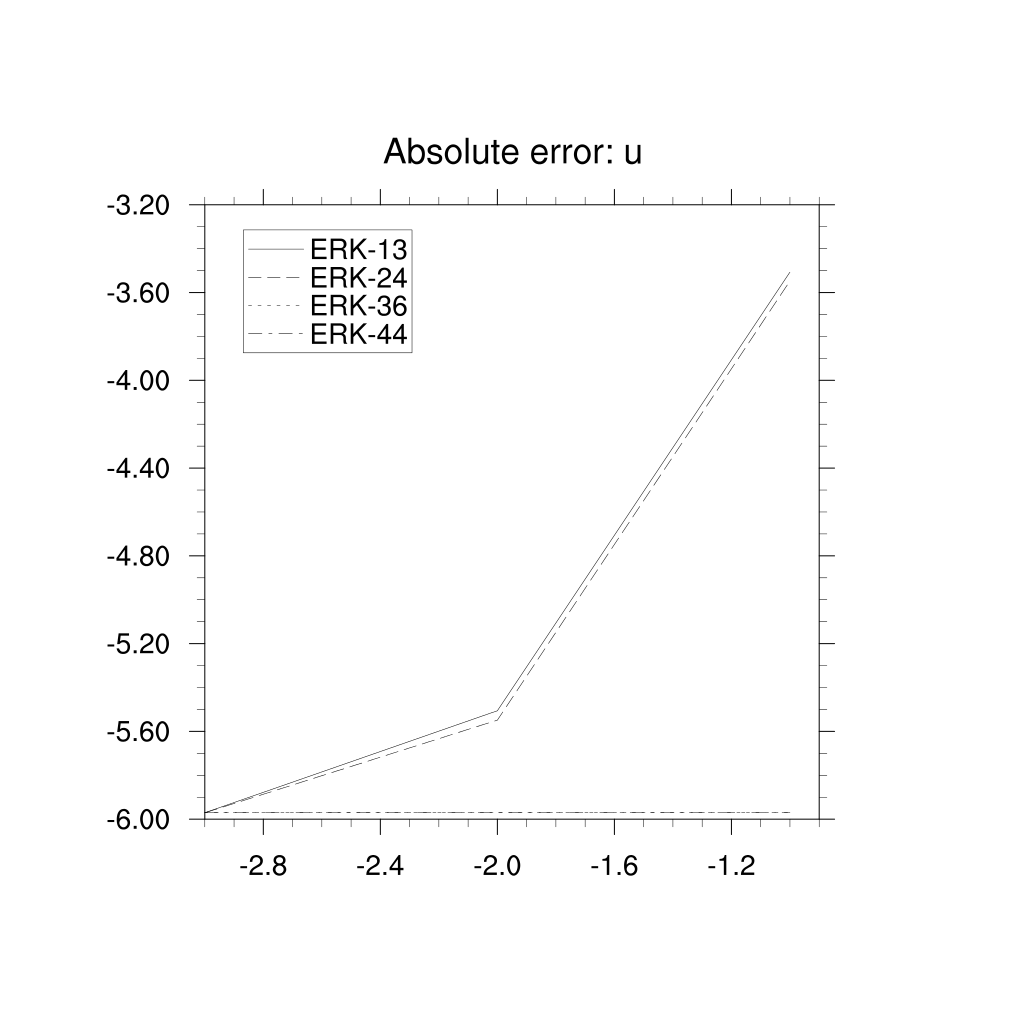
\includegraphics{plots/CFKu_err.png}} 
&
\scalebox{0.15}{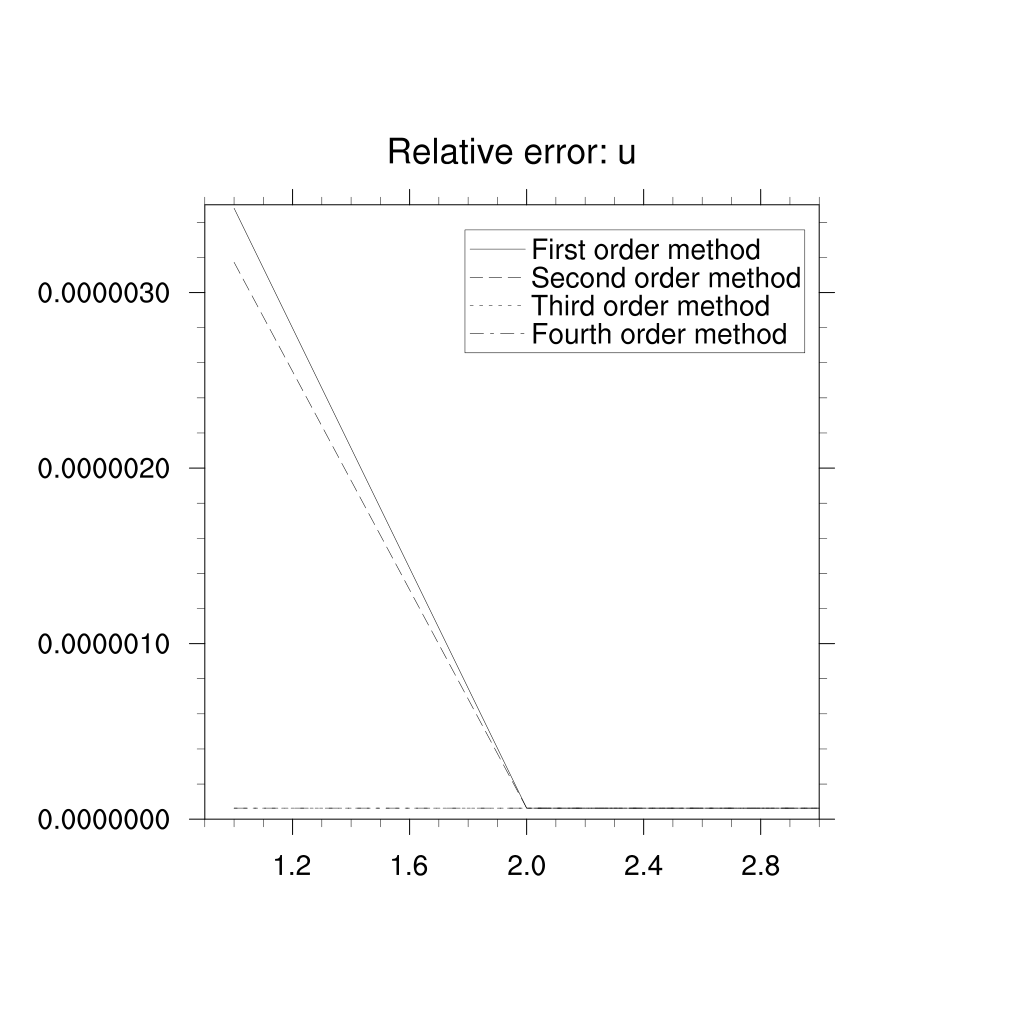
\includegraphics{plots/CFKu_err_rel.png}}
\\
\scalebox{0.15}{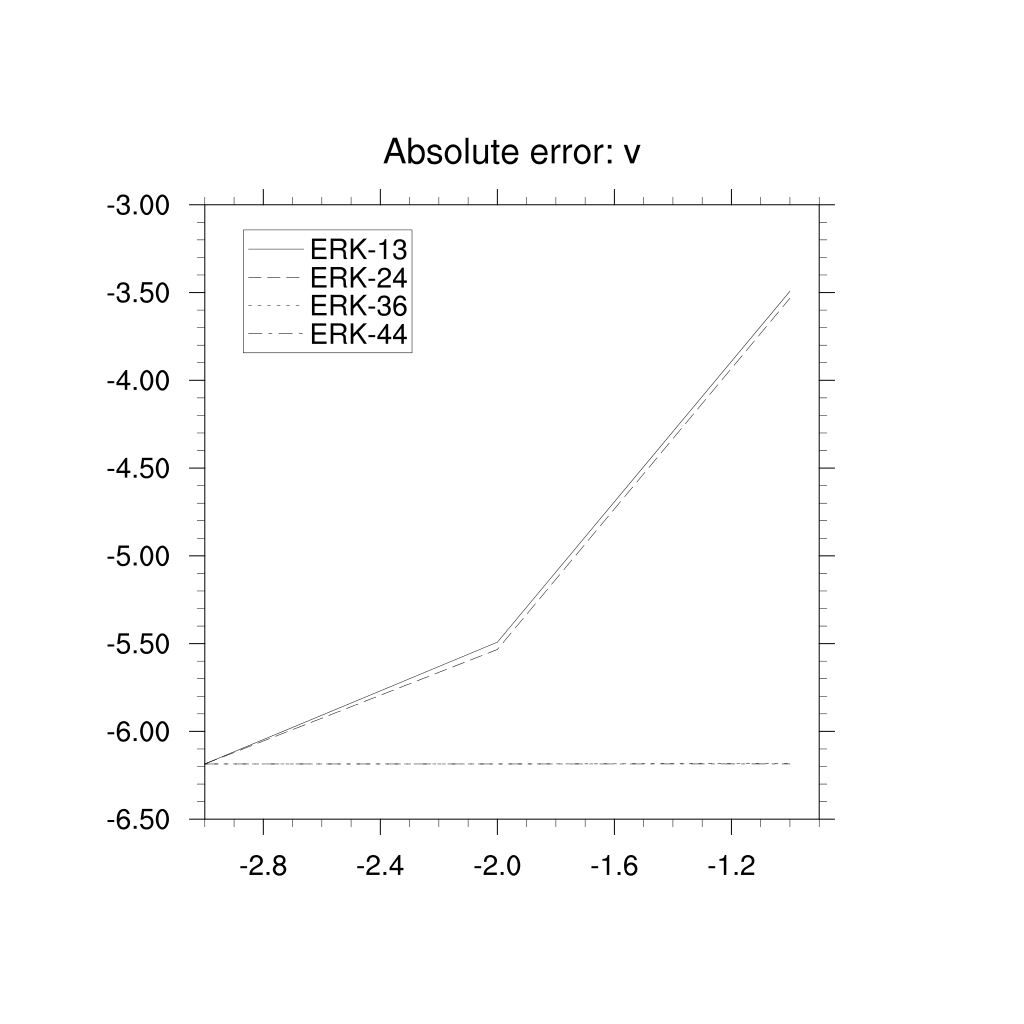
\includegraphics{plots/CFKv_err.png}} 
&
\scalebox{0.15}{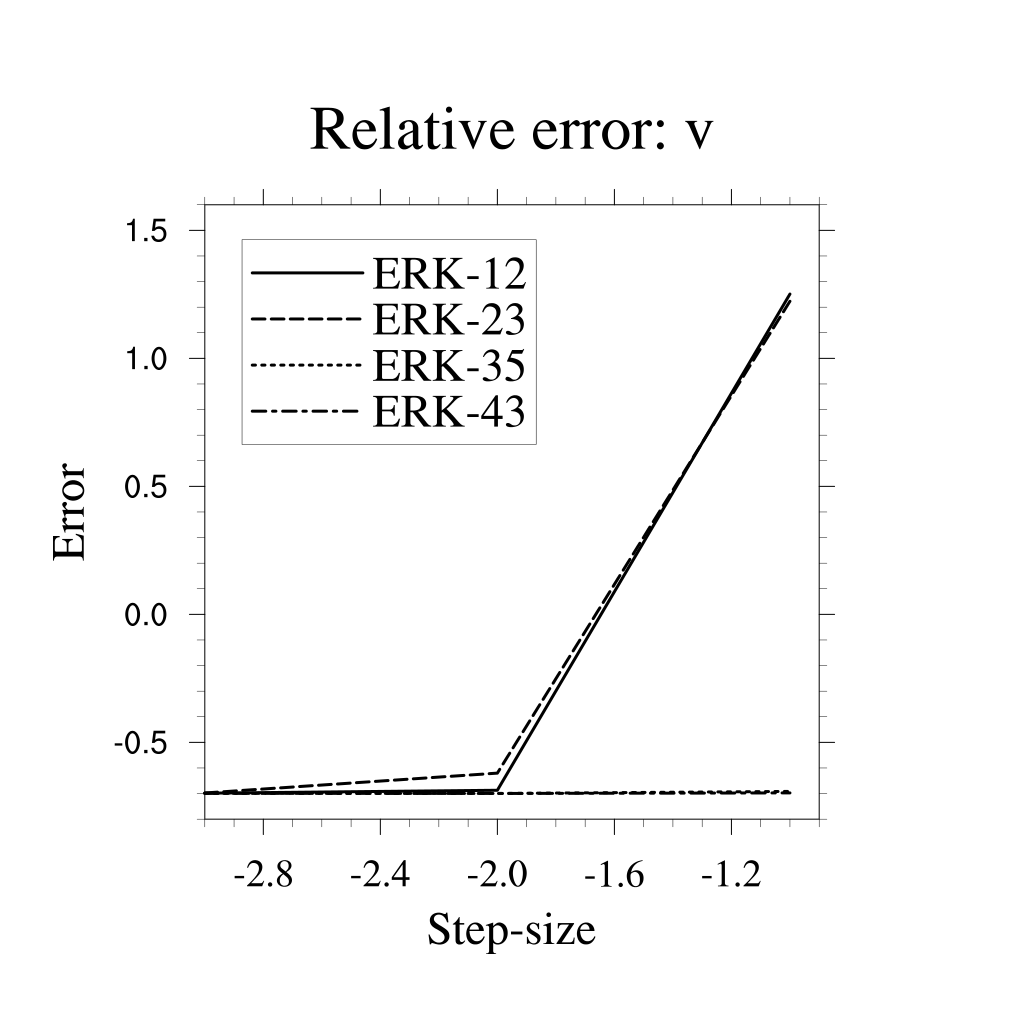
\includegraphics{plots/CFKv_err_rel.png}}
\end{tabular}
\end{center}
\caption{Errors with exponential integrating factor methods.}
\end{figure}

\begin{figure}[hb]
\label{CFK:fig:convtest1}
\begin{center}
\begin{tabular}{cc}
\scalebox{0.15}{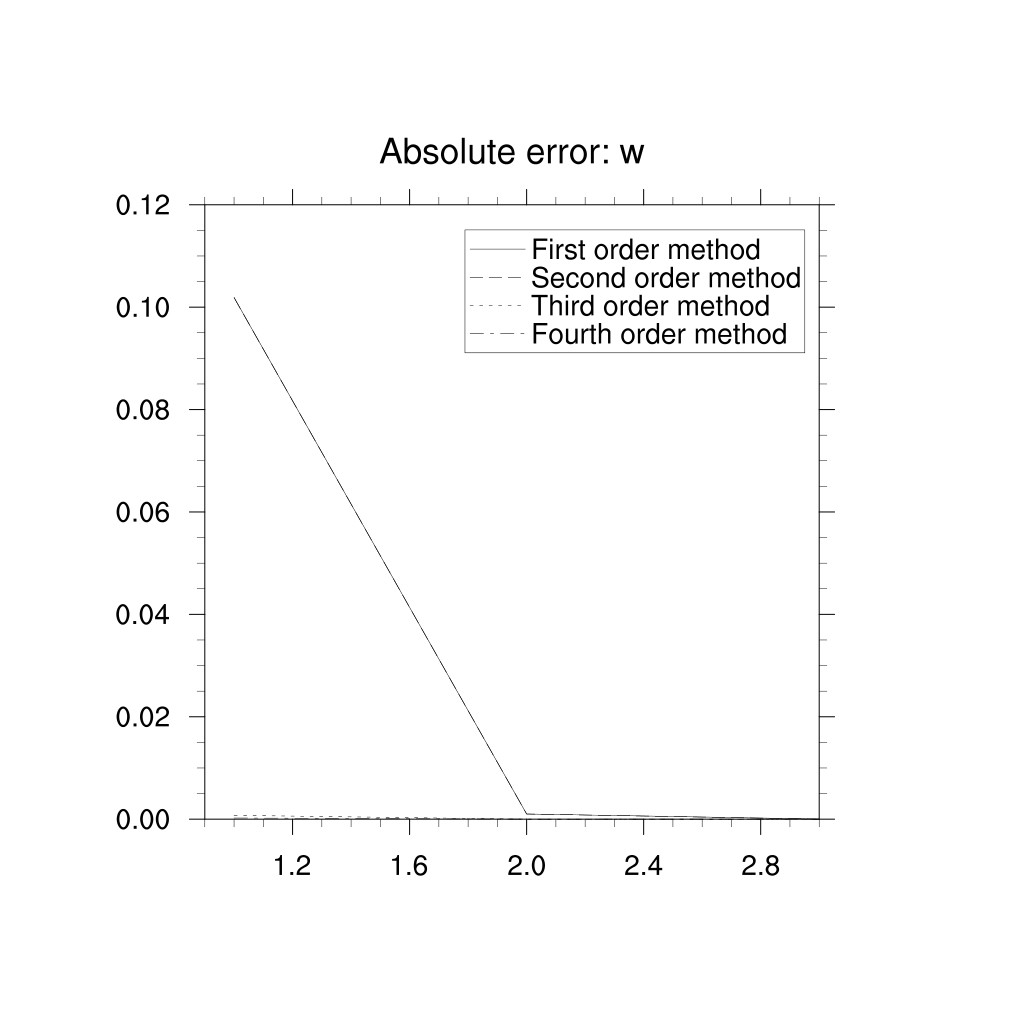
\includegraphics{plots/CFKw_err.png}} 
&
\scalebox{0.15}{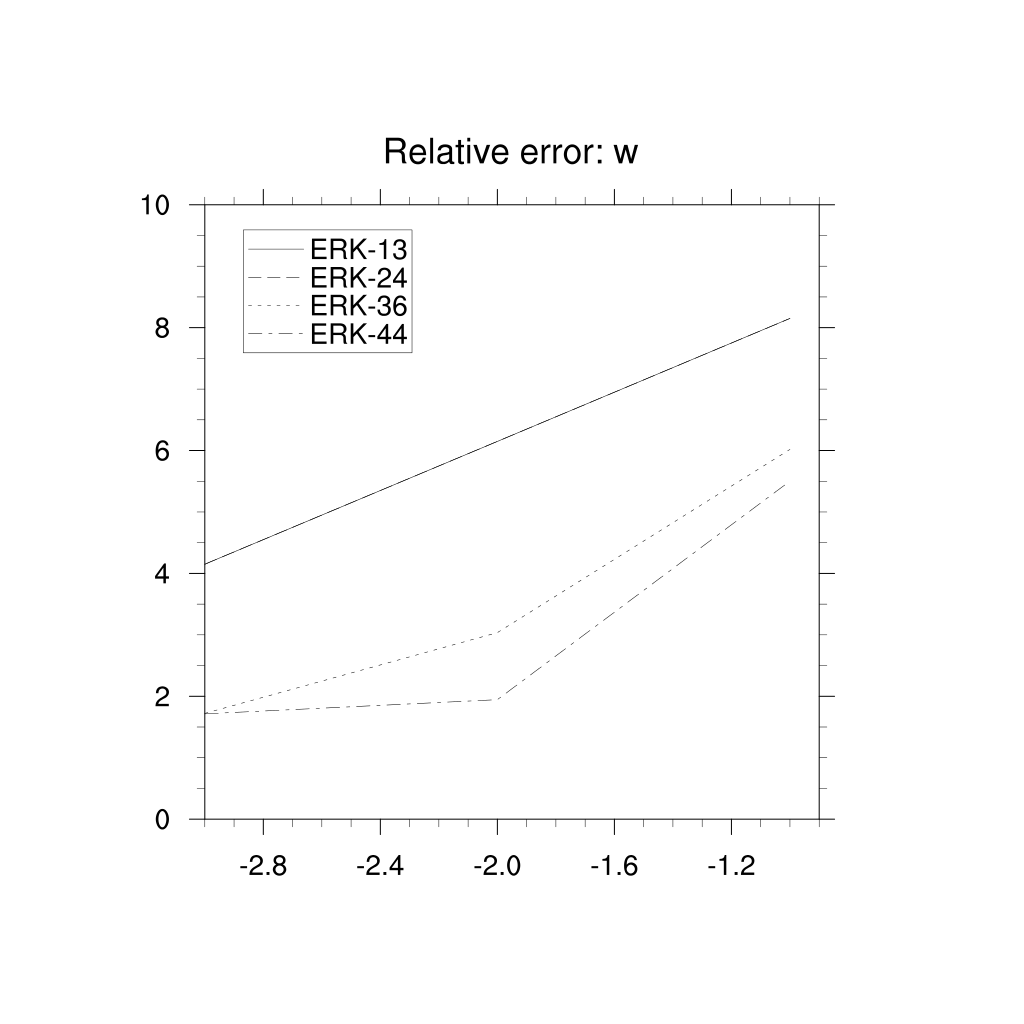
\includegraphics{plots/CFKw_err_rel.png}}
\\
\scalebox{0.15}{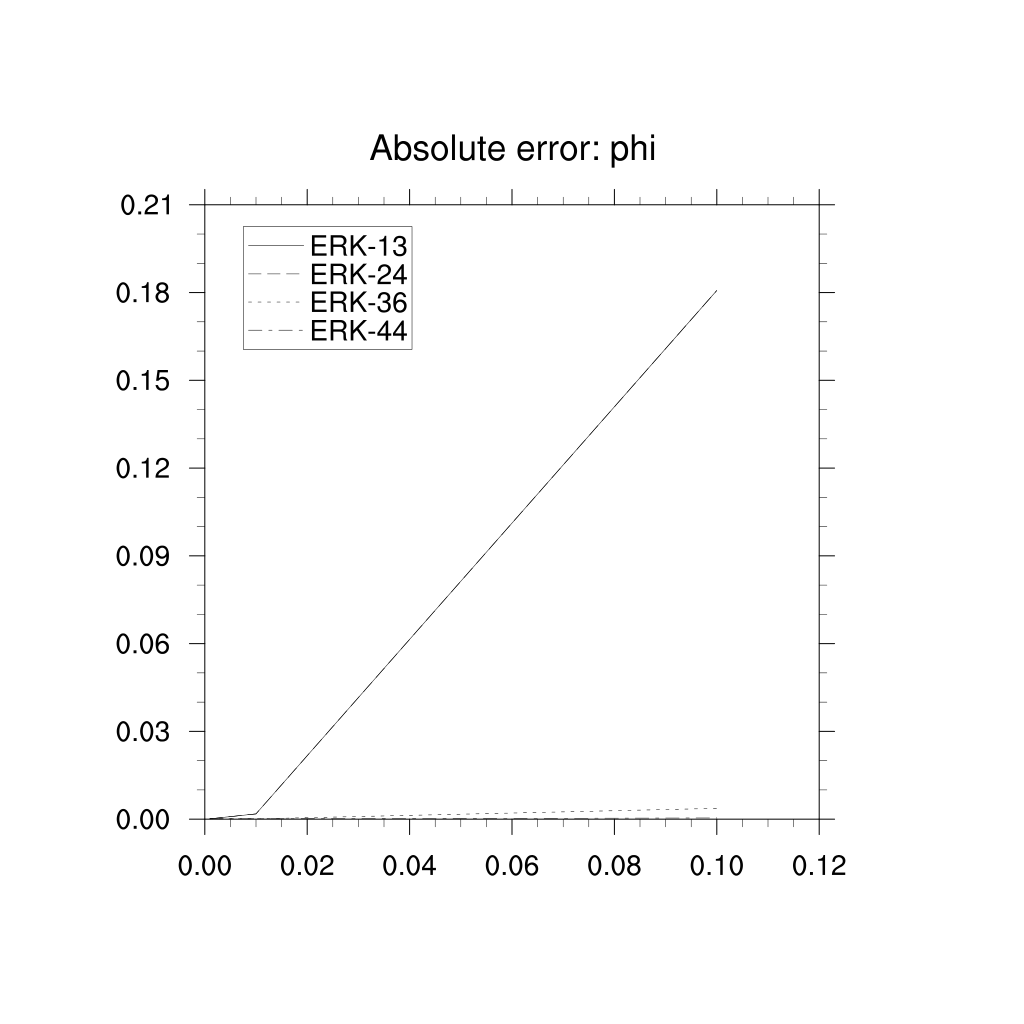
\includegraphics{plots/CFKphi_err.png}} 
&
\scalebox{0.15}{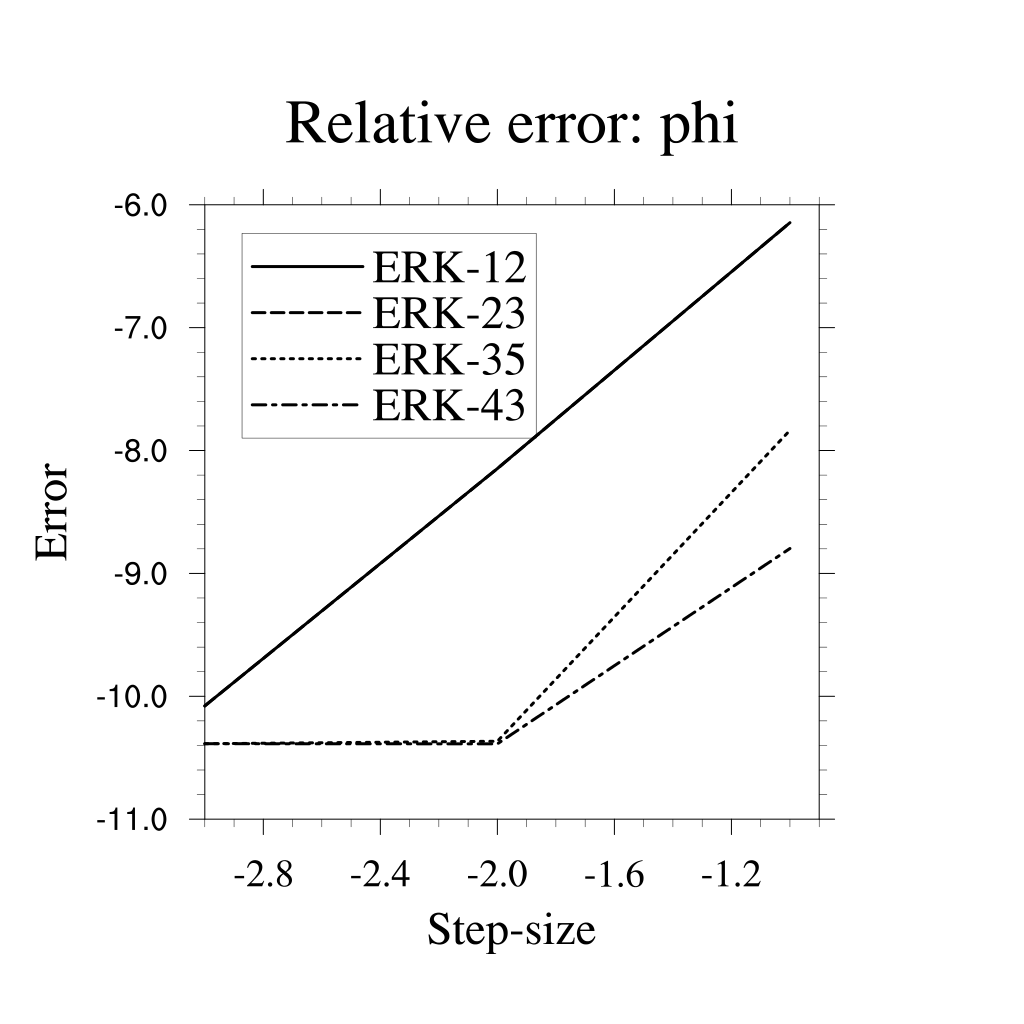
\includegraphics{plots/CFKphi_err_rel.png}}
\end{tabular}
\end{center}
\caption{Errors with exponential integrating factor methods, continued.}
\end{figure}

\section{Conclusions}
Another important matter to take into consideration is that since the 
Jacobian at each point can be computed at the beginning of each time step.
Once we have the Jacobian, the HEVI-Exponential method does not rely 
on neighboring points at all, so we can parallelize this algorithm so that
all of the HEVI-Exponential computations can be done at once.

The HEVI-Exponential approach allows us to deal with stiff initial value
problems with a larger stepsize than a fully explicit method, and the 
opportunity for parallelization with HOMME-NH offers efficiency. Though 
the formation of the matrix exponential can be a costly computation, we 
are able to take advantage of the tridiagonal-like form of the Jacobian in 
HOMME-NH, to implement the HEVI-Exponential methods quite efficiently.

The parallelization of the HEVI-Exponential methods and their direct 
comparison with the IMEX RK methods currently implemented in HOMME-NH 
remains to be studied. This will be further explored an a subsequent paper.

\bibliographystyle{siam}
% Edit the line below to be your first and last names.
\bibliography{CassidyKrause}

% Edit FirstnameLastname below to be your first and last names, but leave the line commented out.
% This line will help me merge bibliographies for the proceedings.
%\documentclass{csri19}

%%% Starting page will be changed when we combine the proceedings
\setcounter{page}{3}

% PACKAGES ---------------------------------------------------------------
\usepackage{amsfonts,amsmath,graphicx,subfigure}
% ADD YOUR OWN PACKAGES HERE ---------------------------------------------
\usepackage{mathtools, amssymb}

% DEFINITIONS ------------------------------------------------------------
% ADD YOUR OWN DEFINITIONS HERE ------------------------------------------
% BE SURE TO PREFACE LABEL WITH YOUR OWN INITIALS (SSS in this example) --
\newcommand{\SSSnorm}[1]{\left\Vert#1\right\Vert}
\newcommand{\SSSabs}[1]{\left\vert#1\right\vert}
\newcommand{\CFKg}{\mathfrak{g}}

% This controls the table-of-contents entry in the proceedings. Edit it
% to include your article title followed by the authors' names, as shown.
\addcontentsline{toc}{chapter}{Exponential Integrators for the Energy Exascale Earth System Model\\
{\em C.F.\ Krause and A.J.\ Steyer}}

\pagestyle{myheadings}

\thispagestyle{plain}

% This gives the running head. Usually you list a shortened version of
% your article title (unless it's already very short) along with
% the author's names, as shown.
\markboth{Exponential Integrators for E3SM}{C.F.\ Krause and A.J.\ Steyer}

% Put your article title in here
\title{Exponential Integrators for the Energy Exascale Earth System Model}

% List each author, their affiliation, and their e-mail address, as shown.
\author{Cassidy F.\ Krause\thanks{University of Kansas, ckrause@ku.edu} \and Andrew J.\ Steyer\thanks{Sandia National Laboratories,
asteyer@sandia.gov}}

\begin{document}



\maketitle

% Include your abstract here.
\begin{abstract}
The HOMME-NH nonhydrostatic atmosphere model has a system of stiff ODEs, which are currently solved in an implicit-explicit (IMEX) Runge-Kutta (RK) methods. We investigate the use of exponential-type integrators to solve these stiff equations, and study their performance.
\end{abstract}

\section{Introduction} \label{CFK:sec:intro}
Stiff ODEs are notorious for requiring a very small step size when solved explicitly. Because this restriction can make algorithms quite inefficient, two different methods have been developed for dealing with these problems. 

Suppose we have an ODE given by 
\[ f(u) = s(u) + n(u),\] where $s(u)$ contains the stiff part of the equation, and $n(u)$ contains the nonstiff part. 
One way to deal with this problem is to use an implicit Runge-Kutta method on the stiff part, and an explicit Runge-Kutta on the nonstiff part. 
This is the current method used in the HOMME-NH nonhydrostatic atmosphere model of the E3SM, and it performs quite well.

Another approach is to use an exponential-type integrator, such as integrating factor Runge-Kutta methods (IFRKs). In this case, we split our method as
\[ f(u) = Lu + N(u),\] where $L$ is a linear operator containing the stiff part of the ODE, and $N(u) = f(u) - Lu$ contains the nonstiff terms. Often, $L = f'(u)$, but we do not assume this is the case. 

Using the change of variables $v(t) = e^{-L(t-t_m)}u(t)$, we have
\begin{equation}\label{CFK:eqn:transformation}
v_t = e^{-L(t-t_m)}N(e^{L(t-t_m)}v).
\end{equation} 
We can then apply an $r-$stage Runge-Kutta method to solve \ref{CFK:eqn:transformation}. In this paper, we implement these exponential-type methods in the HOMME-NH model as a feasible alternative to the IMEX Runge-Kutta methods.

The rest of the paper is structured as follows: In section \ref{CFK:sec:homme}, we give a brief background of the non-hydrostatic model; 
section \ref{CFK:sec:matexp} discusses exponential integrator methods; and numerical results are given in section \ref{CFK:sec:results}

\section{HOMME-NH}\label{CFK:sec:homme}
In the HOMME-NH model, we employ a horizontally explicit, vertically implicit (HEVI) partitioning. Choosing to linearize around the stiffly treated terms, we can write the governing equations as
\[q_t \coloneqq \begin{bmatrix} u_t \\
w_t\\
\phi_t\\
\theta_t\\
\frac{\partial \pi}{\partial \eta}
\end{bmatrix} = n(q) + s(q) \equiv n(q) + \begin{bmatrix}
0\\
-\CFKg (1-\mu)\\
\CFKg w\\
0\\
0\end{bmatrix},\] where $w, u,\phi, \theta,$ and $\frac{\partial \pi}{\partial \eta}$ are the state variables in the HOMME-NH model, as listed in table \ref{CFK:tab:variables}.

\begin{table}
  \caption{Variables in HOMME-NH}
  \label{CFK:tab:variables}
  \begin{center}
    \begin{tabular}{|c|l|}
      \hline
      \textbf{Variable Name} & \textbf{Description} \\
      \hline
      $w$ & Vertical velocity \\
      $u$ & \\
      $\phi$ & Geopotential \\
      $\theta$ & Potential temperature \\
      $\frac{\partial\pi}{\partial\eta}$ & \\
      \hline 
    \end{tabular}
  \end{center}
\end{table}

Linearizing $s(q)$ gives the following Jacobian:
\[ J = \begin{bmatrix}
 &                  &                                                   &  & \\
 & 0                & \CFKg \Delta t \frac{\partial \mu}{\partial \phi} &  & \\
 & \CFKg \Delta t I & 0                                                 &  & \\
 &                  &                                                   &  & \\
 &                  &                                                   &  & \end{bmatrix}.\]

So, forming $e^{\alpha J}$ reduces to forming an exponential of 
\[ \begin{bmatrix}
   0              & \CFKg \Delta t \frac{\partial \mu}{\partial \phi} \\
 \CFKg \Delta t I & 0  \end{bmatrix},\]
where $\dfrac{\partial \mu}{\partial \phi}$ is tridiagonal. The most computationally expensive part of exponential-type methods is forming the matrix exponential; 
as discussed in the next section, we are able to leverage the structure of this particular Jacobian in order to develop methods that are competitive with the currently implemented IMEX Runge-Kutta methods.

\subsection{The Matrix Exponential}\label{CFK:sec:matexp} 
One can form the matrix exponential analytically if the matrix $A$ is diagonalizable, but finding the eigenvalues of $A$ is expensive, and it is not generally guaranteed that $A$ is diagonalizable.
A more general approach is to approximate $e^{A}$ using a Pad\'e or Taylor series approximation. Other methods of approximating the matrix exponential are discussed in \cite{CFK:Moler2003}.

We choose to implement a $(p,q)$ Pad\'e approximation $e^{A}\approx \left[Q_{pq}(A)\right]^{-1}P_{pq}(A)$, where $P_{pq}(A)$ and $Q_{pq}(A)$ are defined as follows:
\begin{align*}
P_{pq}(A) &= \sum_{j=1}^p\frac{(p+q-j)!p!}{(p+q)!j!(p-j)!}A^j\\
Q_{pq}(A) &= \sum_{j=1}^q\frac{(p+q-j)!q!}{(p+q)!j!(q-j)!}(-A)^j
\end{align*}

The error for this approximation is given by
\[ e^A - \left[Q_{pq}(A)\right]^{-1}P_{pq}(A) = \mathcal{O}(A^{p+q+1}).\]

If the matrix $A$ has eigenvalues that are spread far apart, this approximation can be rather inaccuarate. 
To mitigate this problem, we implement a scaling and squaring approach. Because of the properties of matrix exponentials, we can write
\[e^{A} = \left(e^{A/k}\right)^k,\]
where $k$ is chosen to be the smallest power of $2$ so that $\|A/k\| \leq 0.5$.
With this factorization, the matrix $A$ is scaled down to $A/k$, and the matrix exponential $e^{A/k}$ is calculated using the formulas above. This matrix exponential is then squared repeatedly to recover the desired matrix exponential $e^{A}$.

Once the terms $P_{pq}$ and $Q_{pq}$ are calculated, the product $\left[Q_{pq}(A)\right]^{-1}P_{pq}(A)$ is a potentially expensive computation.
Fortunately, for our problem, the matrix $A$ we consider has a special structure. It is of the form \[A= \begin{bmatrix} 0 & \alpha T\\
  \alpha I & 0 \end{bmatrix},\]
where $T$ is tridiagonal. This form allows us to solve $\left[Q_{pq}(A)\right]^{-1}P_{pq}(A)$ using tridiagonal solves and back substitution.

To do so, we first factor $Q_{pq}(A)$ as
\[ Q_{pq}(A) = \prod_{j=1}^q\left[\sigma_jI-A\right]\text{, where }\sigma_j\in \mathbb{C}\text{ for }j=1,\dots,q.\]

Then, since we want to solve for $R \coloneqq \left[Q_{pq}(A)\right]^{-1}P_{pq}(A)$, we have
\begin{align*}
Q_{pq}(A) R &= P_{pq}(A)\\
\prod_{j=1}^q\left[\sigma_jI-A\right]R &= P_{pq}(A).
\end{align*}

Define $R_1 \coloneqq \left[\sigma_2I-A\right]\left[\sigma_3I-A\right]\cdots\left[\sigma_qI-A\right]R$.
Then our equation becomes
\[ \left[\sigma_1I-A\right]R_1 = P_{pq}(A).\] Since $\left[\sigma_1I-A\right]$ is a tridiagonal matrix, we can solve for $R_1$ using far fewer operations than if $\left[\sigma_1I-A\right]$ were a full matrix.

Now we have
\[\left[\sigma_2I-A\right]\left[\sigma_3I-A\right]\cdots\left[\sigma_qI-A\right]R = R_1.\] We can continue in this way, defining $R_j \coloneqq \left[\sigma_{j+1}I-A\right]\left[\sigma_{j+2}I-A\right]\cdots\left[\sigma_qI-A\right]R$ and solving
\[\left[\sigma_jI-A\right]R_j = R_{j-1}\] for $R_j$, until we arive at
\[\left[\sigma_qI-A\right]R = R_{q-1}.\] Solving this last tridiagonal system gives us the $R = \left[Q_{pq}(A)\right]^{-1}P_{pq}(A)$ that we are looking for.

This approach is particularly efficient if the values of $p$ and $q$ are small, so that we can analytically find $\{\sigma_j\}_{j=1}^q$ ahead of time.
Of course, approximations like this do rather poorly for ill-conditioned matrices, so we must validate that these approximations work for the Jacobians we are interested in.
To validate the Pad\'e approximation, we let the model spin up to $3600$ seconds. The Jacobian we are considering at this time has unique eigenvalues, so we can calculate the matrix exponential analytically, and compare it to our approximation.
The following table gives the results of several Pad\'e approximations, depending on the number of terms used in the series.
\begin{table}[ht]
  \begin{center}
    \caption{Error of Pad\'e Approximation}
    \label{CFK:tab:PadeError}
    \begin{tabular}{|c|c|}
      \hline
      \textbf{Number of Terms} & \textbf{Error}\\
      \hline
      2 & 1.30e-10 \\
      3 & 5.25e-13 \\
      4 & 4.92e-13 \\
      5 & 5.42e-13 \\
      \hline
    \end{tabular}
  \end{center}
\end{table}

Since a (22)-Pad\'e approximation yields a considerably accurate matrix exponential and also gives the benefit of taking advantage of the tridiagonal structure, we choose to implement this method.

\newpage
\section{Results}\label{CFK:sec:results}

\section{Conclusions}

\bibliographystyle{siam}
% Edit the line below to be your first and last names.
\bibliography{CassidyKrause}

% Edit FirstnameLastname below to be your first and last names, but leave the line commented out.
% This line will help me merge bibliographies for the proceedings.
%\documentclass{csri19}

%%% Starting page will be changed when we combine the proceedings
\setcounter{page}{3}

% PACKAGES ---------------------------------------------------------------
\usepackage{amsfonts,amsmath,graphicx,subfigure}
% ADD YOUR OWN PACKAGES HERE ---------------------------------------------
\usepackage{mathtools, amssymb}

% DEFINITIONS ------------------------------------------------------------
% ADD YOUR OWN DEFINITIONS HERE ------------------------------------------
% BE SURE TO PREFACE LABEL WITH YOUR OWN INITIALS (SSS in this example) --
\newcommand{\SSSnorm}[1]{\left\Vert#1\right\Vert}
\newcommand{\SSSabs}[1]{\left\vert#1\right\vert}
\newcommand{\CFKg}{\mathfrak{g}}

% This controls the table-of-contents entry in the proceedings. Edit it
% to include your article title followed by the authors' names, as shown.
\addcontentsline{toc}{chapter}{Exponential Integrators for the Energy Exascale Earth System Model\\
{\em C.F.\ Krause and A.J.\ Steyer}}

\pagestyle{myheadings}

\thispagestyle{plain}

% This gives the running head. Usually you list a shortened version of
% your article title (unless it's already very short) along with
% the author's names, as shown.
\markboth{Exponential Integrators for E3SM}{C.F.\ Krause and A.J.\ Steyer}

% Put your article title in here
\title{Exponential Integrators for the Energy Exascale Earth System Model}

% List each author, their affiliation, and their e-mail address, as shown.
\author{Cassidy F.\ Krause\thanks{University of Kansas, ckrause@ku.edu} \and Andrew J.\ Steyer\thanks{Sandia National Laboratories,
asteyer@sandia.gov}}

\begin{document}



\maketitle

% Include your abstract here.
\begin{abstract}
The HOMME-NH nonhydrostatic atmosphere model has a system of stiff ODEs, which are currently solved in an implicit-explicit (IMEX) Runge-Kutta (RK) methods. We investigate the use of exponential-type integrators to solve these stiff equations, and study their performance.
\end{abstract}

\section{Introduction} \label{CFK:sec:intro}
Stiff ODEs are notorious for requiring a very small step size when solved explicitly. Because this restriction can make algorithms quite inefficient, two different methods have been developed for dealing with these problems. 

Suppose we have an ODE given by 
\[ f(u) = s(u) + n(u),\] where $s(u)$ contains the stiff part of the equation, and $n(u)$ contains the nonstiff part. 
One way to deal with this problem is to use an implicit Runge-Kutta method on the stiff part, and an explicit Runge-Kutta on the nonstiff part. 
This is the current method used in the HOMME-NH nonhydrostatic atmosphere model of the E3SM, and it performs quite well.

Another approach is to use an exponential-type integrator, such as integrating factor Runge-Kutta methods (IFRKs). In this case, we split our method as
\[ f(u) = Lu + N(u),\] where $L$ is a linear operator containing the stiff part of the ODE, and $N(u) = f(u) - Lu$ contains the nonstiff terms. Often, $L = f'(u)$, but we do not assume this is the case. 

Using the change of variables $v(t) = e^{-L(t-t_m)}u(t)$, we have
\begin{equation}\label{CFK:eqn:transformation}
v_t = e^{-L(t-t_m)}N(e^{L(t-t_m)}v).
\end{equation} 
We can then apply an $r-$stage Runge-Kutta method to solve \ref{CFK:eqn:transformation}. In this paper, we implement these exponential-type methods in the HOMME-NH model as a feasible alternative to the IMEX Runge-Kutta methods.

The rest of the paper is structured as follows: In section \ref{CFK:sec:homme}, we give a brief background of the non-hydrostatic model; 
section \ref{CFK:sec:matexp} discusses exponential integrator methods; and numerical results are given in section \ref{CFK:sec:results}

\section{HOMME-NH}\label{CFK:sec:homme}
In the HOMME-NH model, we employ a horizontally explicit, vertically implicit (HEVI) partitioning. Choosing to linearize around the stiffly treated terms, we can write the governing equations as
\[q_t \coloneqq \begin{bmatrix} u_t \\
w_t\\
\phi_t\\
\theta_t\\
\frac{\partial \pi}{\partial \eta}
\end{bmatrix} = n(q) + s(q) \equiv n(q) + \begin{bmatrix}
0\\
-\CFKg (1-\mu)\\
\CFKg w\\
0\\
0\end{bmatrix},\] where $w, u,\phi, \theta,$ and $\frac{\partial \pi}{\partial \eta}$ are the state variables in the HOMME-NH model, as listed in table \ref{CFK:tab:variables}.

\begin{table}
  \caption{Variables in HOMME-NH}
  \label{CFK:tab:variables}
  \begin{center}
    \begin{tabular}{|c|l|}
      \hline
      \textbf{Variable Name} & \textbf{Description} \\
      \hline
      $w$ & Vertical velocity \\
      $u$ & \\
      $\phi$ & Geopotential \\
      $\theta$ & Potential temperature \\
      $\frac{\partial\pi}{\partial\eta}$ & \\
      \hline 
    \end{tabular}
  \end{center}
\end{table}

Linearizing $s(q)$ gives the following Jacobian:
\[ J = \begin{bmatrix}
 &                  &                                                   &  & \\
 & 0                & \CFKg \Delta t \frac{\partial \mu}{\partial \phi} &  & \\
 & \CFKg \Delta t I & 0                                                 &  & \\
 &                  &                                                   &  & \\
 &                  &                                                   &  & \end{bmatrix}.\]

So, forming $e^{\alpha J}$ reduces to forming an exponential of 
\[ \begin{bmatrix}
   0              & \CFKg \Delta t \frac{\partial \mu}{\partial \phi} \\
 \CFKg \Delta t I & 0  \end{bmatrix},\]
where $\dfrac{\partial \mu}{\partial \phi}$ is tridiagonal. The most computationally expensive part of exponential-type methods is forming the matrix exponential; 
as discussed in the next section, we are able to leverage the structure of this particular Jacobian in order to develop methods that are competitive with the currently implemented IMEX Runge-Kutta methods.

\subsection{The Matrix Exponential}\label{CFK:sec:matexp} 
One can form the matrix exponential analytically if the matrix $A$ is diagonalizable, but finding the eigenvalues of $A$ is expensive, and it is not generally guaranteed that $A$ is diagonalizable.
A more general approach is to approximate $e^{A}$ using a Pad\'e or Taylor series approximation. Other methods of approximating the matrix exponential are discussed in \cite{CFK:Moler2003}.

We choose to implement a $(p,q)$ Pad\'e approximation $e^{A}\approx \left[Q_{pq}(A)\right]^{-1}P_{pq}(A)$, where $P_{pq}(A)$ and $Q_{pq}(A)$ are defined as follows:
\begin{align*}
P_{pq}(A) &= \sum_{j=1}^p\frac{(p+q-j)!p!}{(p+q)!j!(p-j)!}A^j\\
Q_{pq}(A) &= \sum_{j=1}^q\frac{(p+q-j)!q!}{(p+q)!j!(q-j)!}(-A)^j
\end{align*}

The error for this approximation is given by
\[ e^A - \left[Q_{pq}(A)\right]^{-1}P_{pq}(A) = \mathcal{O}(A^{p+q+1}).\]

If the matrix $A$ has eigenvalues that are spread far apart, this approximation can be rather inaccuarate. 
To mitigate this problem, we implement a scaling and squaring approach. Because of the properties of matrix exponentials, we can write
\[e^{A} = \left(e^{A/k}\right)^k,\]
where $k$ is chosen to be the smallest power of $2$ so that $\|A/k\| \leq 0.5$.
With this factorization, the matrix $A$ is scaled down to $A/k$, and the matrix exponential $e^{A/k}$ is calculated using the formulas above. This matrix exponential is then squared repeatedly to recover the desired matrix exponential $e^{A}$.

Once the terms $P_{pq}$ and $Q_{pq}$ are calculated, the product $\left[Q_{pq}(A)\right]^{-1}P_{pq}(A)$ is a potentially expensive computation.
Fortunately, for our problem, the matrix $A$ we consider has a special structure. It is of the form \[A= \begin{bmatrix} 0 & \alpha T\\
  \alpha I & 0 \end{bmatrix},\]
where $T$ is tridiagonal. This form allows us to solve $\left[Q_{pq}(A)\right]^{-1}P_{pq}(A)$ using tridiagonal solves and back substitution.

To do so, we first factor $Q_{pq}(A)$ as
\[ Q_{pq}(A) = \prod_{j=1}^q\left[\sigma_jI-A\right]\text{, where }\sigma_j\in \mathbb{C}\text{ for }j=1,\dots,q.\]

Then, since we want to solve for $R \coloneqq \left[Q_{pq}(A)\right]^{-1}P_{pq}(A)$, we have
\begin{align*}
Q_{pq}(A) R &= P_{pq}(A)\\
\prod_{j=1}^q\left[\sigma_jI-A\right]R &= P_{pq}(A).
\end{align*}

Define $R_1 \coloneqq \left[\sigma_2I-A\right]\left[\sigma_3I-A\right]\cdots\left[\sigma_qI-A\right]R$.
Then our equation becomes
\[ \left[\sigma_1I-A\right]R_1 = P_{pq}(A).\] Since $\left[\sigma_1I-A\right]$ is a tridiagonal matrix, we can solve for $R_1$ using far fewer operations than if $\left[\sigma_1I-A\right]$ were a full matrix.

Now we have
\[\left[\sigma_2I-A\right]\left[\sigma_3I-A\right]\cdots\left[\sigma_qI-A\right]R = R_1.\] We can continue in this way, defining $R_j \coloneqq \left[\sigma_{j+1}I-A\right]\left[\sigma_{j+2}I-A\right]\cdots\left[\sigma_qI-A\right]R$ and solving
\[\left[\sigma_jI-A\right]R_j = R_{j-1}\] for $R_j$, until we arive at
\[\left[\sigma_qI-A\right]R = R_{q-1}.\] Solving this last tridiagonal system gives us the $R = \left[Q_{pq}(A)\right]^{-1}P_{pq}(A)$ that we are looking for.

This approach is particularly efficient if the values of $p$ and $q$ are small, so that we can analytically find $\{\sigma_j\}_{j=1}^q$ ahead of time.
Of course, approximations like this do rather poorly for ill-conditioned matrices, so we must validate that these approximations work for the Jacobians we are interested in.
To validate the Pad\'e approximation, we let the model spin up to $3600$ seconds. The Jacobian we are considering at this time has unique eigenvalues, so we can calculate the matrix exponential analytically, and compare it to our approximation.
The following table gives the results of several Pad\'e approximations, depending on the number of terms used in the series.
\begin{table}[ht]
  \begin{center}
    \caption{Error of Pad\'e Approximation}
    \label{CFK:tab:PadeError}
    \begin{tabular}{|c|c|}
      \hline
      \textbf{Number of Terms} & \textbf{Error}\\
      \hline
      2 & 1.30e-10 \\
      3 & 5.25e-13 \\
      4 & 4.92e-13 \\
      5 & 5.42e-13 \\
      \hline
    \end{tabular}
  \end{center}
\end{table}

Since a (22)-Pad\'e approximation yields a considerably accurate matrix exponential and also gives the benefit of taking advantage of the tridiagonal structure, we choose to implement this method.

\newpage
\section{Results}\label{CFK:sec:results}

\section{Conclusions}

\bibliographystyle{siam}
% Edit the line below to be your first and last names.
\bibliography{CassidyKrause}

% Edit FirstnameLastname below to be your first and last names, but leave the line commented out.
% This line will help me merge bibliographies for the proceedings.
%\documentclass{csri19}

%%% Starting page will be changed when we combine the proceedings
\setcounter{page}{3}

% PACKAGES ---------------------------------------------------------------
\usepackage{amsfonts,amsmath,graphicx,subfigure}
% ADD YOUR OWN PACKAGES HERE ---------------------------------------------
\usepackage{mathtools, amssymb}

% DEFINITIONS ------------------------------------------------------------
% ADD YOUR OWN DEFINITIONS HERE ------------------------------------------
% BE SURE TO PREFACE LABEL WITH YOUR OWN INITIALS (SSS in this example) --
\newcommand{\SSSnorm}[1]{\left\Vert#1\right\Vert}
\newcommand{\SSSabs}[1]{\left\vert#1\right\vert}
\newcommand{\CFKg}{\mathfrak{g}}

% This controls the table-of-contents entry in the proceedings. Edit it
% to include your article title followed by the authors' names, as shown.
\addcontentsline{toc}{chapter}{Exponential Integrators for the Energy Exascale Earth System Model\\
{\em C.F.\ Krause and A.J.\ Steyer}}

\pagestyle{myheadings}

\thispagestyle{plain}

% This gives the running head. Usually you list a shortened version of
% your article title (unless it's already very short) along with
% the author's names, as shown.
\markboth{Exponential Integrators for E3SM}{C.F.\ Krause and A.J.\ Steyer}

% Put your article title in here
\title{Exponential Integrators for the Energy Exascale Earth System Model}

% List each author, their affiliation, and their e-mail address, as shown.
\author{Cassidy F.\ Krause\thanks{University of Kansas, ckrause@ku.edu} \and Andrew J.\ Steyer\thanks{Sandia National Laboratories,
asteyer@sandia.gov}}

\begin{document}



\maketitle

% Include your abstract here.
\begin{abstract}
The HOMME-NH nonhydrostatic atmosphere model has a system of stiff ODEs, which are currently solved in an implicit-explicit (IMEX) Runge-Kutta (RK) methods. We investigate the use of exponential-type integrators to solve these stiff equations, and study their performance.
\end{abstract}

\section{Introduction} \label{CFK:sec:intro}
Stiff ODEs are notorious for requiring a very small step size when solved explicitly. Because this restriction can make algorithms quite inefficient, two different methods have been developed for dealing with these problems. 

Suppose we have an ODE given by 
\[ f(u) = s(u) + n(u),\] where $s(u)$ contains the stiff part of the equation, and $n(u)$ contains the nonstiff part. 
One way to deal with this problem is to use an implicit Runge-Kutta method on the stiff part, and an explicit Runge-Kutta on the nonstiff part. 
This is the current method used in the HOMME-NH nonhydrostatic atmosphere model of the E3SM, and it performs quite well.

Another approach is to use an exponential-type integrator, such as integrating factor Runge-Kutta methods (IFRKs). In this case, we split our method as
\[ f(u) = Lu + N(u),\] where $L$ is a linear operator containing the stiff part of the ODE, and $N(u) = f(u) - Lu$ contains the nonstiff terms. Often, $L = f'(u)$, but we do not assume this is the case. 

Using the change of variables $v(t) = e^{-L(t-t_m)}u(t)$, we have
\begin{equation}\label{CFK:eqn:transformation}
v_t = e^{-L(t-t_m)}N(e^{L(t-t_m)}v).
\end{equation} 
We can then apply an $r-$stage Runge-Kutta method to solve \ref{CFK:eqn:transformation}. In this paper, we implement these exponential-type methods in the HOMME-NH model as a feasible alternative to the IMEX Runge-Kutta methods.

The rest of the paper is structured as follows: In section \ref{CFK:sec:homme}, we give a brief background of the non-hydrostatic model; 
section \ref{CFK:sec:matexp} discusses exponential integrator methods; and numerical results are given in section \ref{CFK:sec:results}

\section{HOMME-NH}\label{CFK:sec:homme}
In the HOMME-NH model, we employ a horizontally explicit, vertically implicit (HEVI) partitioning. Choosing to linearize around the stiffly treated terms, we can write the governing equations as
\[q_t \coloneqq \begin{bmatrix} u_t \\
w_t\\
\phi_t\\
\theta_t\\
\frac{\partial \pi}{\partial \eta}
\end{bmatrix} = n(q) + s(q) \equiv n(q) + \begin{bmatrix}
0\\
-\CFKg (1-\mu)\\
\CFKg w\\
0\\
0\end{bmatrix},\] where $w, u,\phi, \theta,$ and $\frac{\partial \pi}{\partial \eta}$ are the state variables in the HOMME-NH model, as listed in table \ref{CFK:tab:variables}.

\begin{table}
  \caption{Variables in HOMME-NH}
  \label{CFK:tab:variables}
  \begin{center}
    \begin{tabular}{|c|l|}
      \hline
      \textbf{Variable Name} & \textbf{Description} \\
      \hline
      $w$ & Vertical velocity \\
      $u$ & \\
      $\phi$ & Geopotential \\
      $\theta$ & Potential temperature \\
      $\frac{\partial\pi}{\partial\eta}$ & \\
      \hline 
    \end{tabular}
  \end{center}
\end{table}

Linearizing $s(q)$ gives the following Jacobian:
\[ J = \begin{bmatrix}
 &                  &                                                   &  & \\
 & 0                & \CFKg \Delta t \frac{\partial \mu}{\partial \phi} &  & \\
 & \CFKg \Delta t I & 0                                                 &  & \\
 &                  &                                                   &  & \\
 &                  &                                                   &  & \end{bmatrix}.\]

So, forming $e^{\alpha J}$ reduces to forming an exponential of 
\[ \begin{bmatrix}
   0              & \CFKg \Delta t \frac{\partial \mu}{\partial \phi} \\
 \CFKg \Delta t I & 0  \end{bmatrix},\]
where $\dfrac{\partial \mu}{\partial \phi}$ is tridiagonal. The most computationally expensive part of exponential-type methods is forming the matrix exponential; 
as discussed in the next section, we are able to leverage the structure of this particular Jacobian in order to develop methods that are competitive with the currently implemented IMEX Runge-Kutta methods.

\subsection{The Matrix Exponential}\label{CFK:sec:matexp} 
One can form the matrix exponential analytically if the matrix $A$ is diagonalizable, but finding the eigenvalues of $A$ is expensive, and it is not generally guaranteed that $A$ is diagonalizable.
A more general approach is to approximate $e^{A}$ using a Pad\'e or Taylor series approximation. Other methods of approximating the matrix exponential are discussed in \cite{CFK:Moler2003}.

We choose to implement a $(p,q)$ Pad\'e approximation $e^{A}\approx \left[Q_{pq}(A)\right]^{-1}P_{pq}(A)$, where $P_{pq}(A)$ and $Q_{pq}(A)$ are defined as follows:
\begin{align*}
P_{pq}(A) &= \sum_{j=1}^p\frac{(p+q-j)!p!}{(p+q)!j!(p-j)!}A^j\\
Q_{pq}(A) &= \sum_{j=1}^q\frac{(p+q-j)!q!}{(p+q)!j!(q-j)!}(-A)^j
\end{align*}

The error for this approximation is given by
\[ e^A - \left[Q_{pq}(A)\right]^{-1}P_{pq}(A) = \mathcal{O}(A^{p+q+1}).\]

If the matrix $A$ has eigenvalues that are spread far apart, this approximation can be rather inaccuarate. 
To mitigate this problem, we implement a scaling and squaring approach. Because of the properties of matrix exponentials, we can write
\[e^{A} = \left(e^{A/k}\right)^k,\]
where $k$ is chosen to be the smallest power of $2$ so that $\|A/k\| \leq 0.5$.
With this factorization, the matrix $A$ is scaled down to $A/k$, and the matrix exponential $e^{A/k}$ is calculated using the formulas above. This matrix exponential is then squared repeatedly to recover the desired matrix exponential $e^{A}$.

Once the terms $P_{pq}$ and $Q_{pq}$ are calculated, the product $\left[Q_{pq}(A)\right]^{-1}P_{pq}(A)$ is a potentially expensive computation.
Fortunately, for our problem, the matrix $A$ we consider has a special structure. It is of the form \[A= \begin{bmatrix} 0 & \alpha T\\
  \alpha I & 0 \end{bmatrix},\]
where $T$ is tridiagonal. This form allows us to solve $\left[Q_{pq}(A)\right]^{-1}P_{pq}(A)$ using tridiagonal solves and back substitution.

To do so, we first factor $Q_{pq}(A)$ as
\[ Q_{pq}(A) = \prod_{j=1}^q\left[\sigma_jI-A\right]\text{, where }\sigma_j\in \mathbb{C}\text{ for }j=1,\dots,q.\]

Then, since we want to solve for $R \coloneqq \left[Q_{pq}(A)\right]^{-1}P_{pq}(A)$, we have
\begin{align*}
Q_{pq}(A) R &= P_{pq}(A)\\
\prod_{j=1}^q\left[\sigma_jI-A\right]R &= P_{pq}(A).
\end{align*}

Define $R_1 \coloneqq \left[\sigma_2I-A\right]\left[\sigma_3I-A\right]\cdots\left[\sigma_qI-A\right]R$.
Then our equation becomes
\[ \left[\sigma_1I-A\right]R_1 = P_{pq}(A).\] Since $\left[\sigma_1I-A\right]$ is a tridiagonal matrix, we can solve for $R_1$ using far fewer operations than if $\left[\sigma_1I-A\right]$ were a full matrix.

Now we have
\[\left[\sigma_2I-A\right]\left[\sigma_3I-A\right]\cdots\left[\sigma_qI-A\right]R = R_1.\] We can continue in this way, defining $R_j \coloneqq \left[\sigma_{j+1}I-A\right]\left[\sigma_{j+2}I-A\right]\cdots\left[\sigma_qI-A\right]R$ and solving
\[\left[\sigma_jI-A\right]R_j = R_{j-1}\] for $R_j$, until we arive at
\[\left[\sigma_qI-A\right]R = R_{q-1}.\] Solving this last tridiagonal system gives us the $R = \left[Q_{pq}(A)\right]^{-1}P_{pq}(A)$ that we are looking for.

This approach is particularly efficient if the values of $p$ and $q$ are small, so that we can analytically find $\{\sigma_j\}_{j=1}^q$ ahead of time.
Of course, approximations like this do rather poorly for ill-conditioned matrices, so we must validate that these approximations work for the Jacobians we are interested in.
To validate the Pad\'e approximation, we let the model spin up to $3600$ seconds. The Jacobian we are considering at this time has unique eigenvalues, so we can calculate the matrix exponential analytically, and compare it to our approximation.
The following table gives the results of several Pad\'e approximations, depending on the number of terms used in the series.
\begin{table}[ht]
  \begin{center}
    \caption{Error of Pad\'e Approximation}
    \label{CFK:tab:PadeError}
    \begin{tabular}{|c|c|}
      \hline
      \textbf{Number of Terms} & \textbf{Error}\\
      \hline
      2 & 1.30e-10 \\
      3 & 5.25e-13 \\
      4 & 4.92e-13 \\
      5 & 5.42e-13 \\
      \hline
    \end{tabular}
  \end{center}
\end{table}

Since a (22)-Pad\'e approximation yields a considerably accurate matrix exponential and also gives the benefit of taking advantage of the tridiagonal structure, we choose to implement this method.

\newpage
\section{Results}\label{CFK:sec:results}

\section{Conclusions}

\bibliographystyle{siam}
% Edit the line below to be your first and last names.
\bibliography{CassidyKrause}

% Edit FirstnameLastname below to be your first and last names, but leave the line commented out.
% This line will help me merge bibliographies for the proceedings.
%\input{CassidyKrause.bbl}

\end{document}


\end{document}


\end{document}


\end{document}
